%%%%%%%%%%%%%%%%%%%%%%%%%%%%%%%%%%%%%%%%%%%%%%%%%%%%%%%%%%%%%%%%%%%%%%%%%%%%%%%%
%2345678901234567890123456789012345678901234567890123456789012345678901234567890
%        1         2         3         4         5         6         7         8

\documentclass[letterpaper, 10 pt, conference]{ieeeconf}  % Comment this line out if you need a4paper

%\documentclass[a4paper, 10pt, conference]{ieeeconf}      % Use this line for a4 paper

\IEEEoverridecommandlockouts                              % This command is only needed if 
                                                          % you want to use the \thanks command

\overrideIEEEmargins                                      % Needed to meet printer requirements.

%In case you encounter the following error:
%Error 1010 The PDF file may be corrupt (unable to open PDF file) OR
%Error 1000 An error occurred while parsing a contents stream. Unable to analyze the PDF file.
%This is a known problem with pdfLaTeX conversion filter. The file cannot be opened with acrobat reader
%Please use one of the alternatives below to circumvent this error by uncommenting one or the other
%\pdfobjcompresslevel=0
%\pdfminorversion=4

% See the \addtolength command later in the file to balance the column lengths
% on the last page of the document

% The following packages can be found on http:\\www.ctan.org
%\usepackage{graphics} % for pdf, bitmapped graphics files
%\usepackage{epsfig} % for postscript graphics files
%\usepackage{mathptmx} % assumes new font selection scheme installed
%\usepackage{times} % assumes new font selection scheme installed
%\usepackage{amsmath} % assumes amsmath package installed
%\usepackage{amssymb}  % assumes amsmath package installed

\usepackage{graphicx}
\usepackage{amssymb}
\usepackage{graphicx}
\usepackage{amsmath,amssymb,latexsym,float,epsfig,subfigure}
\usepackage{mathtools, bbm}
\usepackage{amsmath} % assumes amsmath package installed
\usepackage{amssymb}  % assumes amsmath package installed
\usepackage{lipsum}
\usepackage[export]{adjustbox}
\usepackage[normalem]{ulem} % underline
\usepackage{wrapfig}
\usepackage{multirow}
\usepackage{balance}
\usepackage{color}
\usepackage{url}
\usepackage{microtype}
\usepackage{algorithm, algorithmic}
\usepackage{breqn}
\usepackage[bottom]{footmisc}

\newcommand{\argmax}{\arg\!\max}
\newcommand{\norm}[1]{\left\lVert#1\right\rVert}

\title{\LARGE \bf
Information Theoretic Characterization of Human-Robot Interaction using Transfer Entropy
}


\author{Deepak Gopinath$^{1}$ and Brenna D. Argall$^{2}$% <-this % stops a space
\thanks{This material is based upon work supported by the National Science Foundation under Grant CNS 1544741. Any opinions, findings and conclusions or
	recommendations expressed in this material are those of the authors and do
	not necessarily reflect the views of the aforementioned institutions. Deepak Gopinath would also like to thank Dr. Vishnu Sreekumar for initial conversations on transfer entropy.
}% <-this % stops a space
\thanks{$^{1}$ Deepak Gopinath is with the Department of Mechanical Engineering, Northwestern University, Evanston, IL, USA and Shirley Ryan AbilityLab, Chicago, IL, USA
        {\tt\small deepak.gopinath@u.northwestern.edu}}%
\thanks{$^{2}$Brenna D. Argall is with the Department of Mechanical Engineering, Department of Electrical Engineering and Computer Science, Northwestern University, Evanston, IL, Department of Physical Medicine and Rehabilitation, Northwestern University, Chicago, IL and Shirley Ryan AbilityLab, Chicago, IL.
        {\tt\small brenna.argall@northwestern.edu}}%
}


\begin{document}

\maketitle
\thispagestyle{empty}
\pagestyle{empty}


%%%%%%%%%%%%%%%%%%%%%%%%%%%%%%%%%%%%%%%%%%%%%%%%%%%%%%%%%%%%%%%%%%%%%%%%%%%%%%%%
\begin{abstract}
Understanding the dynamics of information flow and exchange between humans and robots is critical for the quantification and design of seamless, fluid and intuitive human-robot interaction paradigms. Information theoretic characterization can lead to novel approaches to the design of robot behaviors that can likely optimize subjective aspects such as user satisfaction and acceptance as well as objective task performance related metrics such as success rate and effort simultaneously. In this paper we characterize the information dynamics of human-robot interaction in a shared-control assistive robotic manipulation setting using the information theoretic concept of \textit{transfer entropy}. Specifically, we consider information flow as quantified by transfer entropy between various time-series signals such as human control commands, robot autonomy commands and goal probabilities. Preliminary results indicate the presence of information flow from the robot to the human and not vice-versa. This indicates that extensive training is important for humans to be able to successfully cooperate and coordinate with robots in task execution (will change upon proper analysis). 
\end{abstract}


%%%%%%%%%%%%%%%%%%%%%%%%%%%%%%%%%%%%%%%%%%%%%%%%%%%%%%%%%%%%%%%%%%%%%%%%%%%%%%%%
\section{INTRODUCTION}

In 1948 Claude Shannon originally proposed \textit{information theory} as a mathematical theory of communication to primarily understand the fundamental limitations of a communication channel and what constitutes optimal data encoding~\cite{shannon2001mathematical}. Shannon's work introduced a mathematically sound and meaningful approach to quantify and think about communication (or flow) of information and has had a profound impact on the emergence of the information era which ushered in the late 20th century, Life in modern society is characterized by the constant generation, exchange, storage and modification of information at a massive scale (for example, multimedia content in social media networks on the world wide web). Shannon's original theory contains all the essential ingredients that are necessary to quantify the information dynamics between various interacting components of such complex systems and can reveal numerous trends and patterns in these interactions. The mathematical formulation of information theory is fundamentally based on statistics of random variables. Information theory, therefore, provides a domain-agnostic mathematical framework to understand the information flow and exchange between dynamical systems and has been widely used in diverse domains such as economics~\cite{maasoumi1993compendium}, neuroscience~\cite{wibral2014directed}, weather forecasting~\cite{kleeman2007information} and even animal-robot interactions~\cite{butail2014information}. More specifically, time series analysis based on information theory has been able to shed light on directed causal influence between different components of complex systems~\cite{hlavavckova2007causality}. 

Information processing is deemed to be a necessary requirement for life; a biological agent needs to first acquire relevant information from the environment before taking any actions~\cite{ashby1991requisite}. Drawing inspiration from how biological agents interact with their environment and each other via information exchange we posit that an information theoretic characterization of human-robot interactions can possibly offer a novel way of thinking about the design of robot behaviors. In order to effectively co-inhabit human environments that are unpredictable and uncertain, robot behaviors have to account for human preferences, intentions and needs~\cite{wasson2003user}.  The key to the development of adaptable, robust, seamless and intuitive human-robot interaction paradigms might be closely linked to the control of information flow and exchange between the human and the robot.  

A typical approach to the design of robot autonomy relies on optimization of robot behaviors with respect to predefined set of performance related reward functions~\cite{kalakrishnan2011stomp}. These reward functions are usually context-specific and as a result the robot behaviors can suffer from generalization issues. A more overarching and encompassing approach that can possibly lead to more adaptable and robust interactions might be one that optimizes for information transfer and processing in a human-robot team. Efficient information transfer can lead to efficient communication and as a consequence will possibly enable the robot to deal with a wider variety of situations using a single core underlying approach.  

As a first step towards an information theoretic approach to the design of robot behavior for human-robot teams, it is imperative to characterize the information \textit{transfer} within a joint human-robot setting in concrete mathematical terms. In this paper we utilize the information theoretic concept of \textit{transfer entropy} to characterize the information flow in human-robot interaction in the context of a shared-control human-robot setting. Transfer entropy is an information theoretic functional that quantifies how much information does a source random process provides about the state transitions in the target random process.

In Section~\ref{sec:related_work} we provide a brief overview of information theoretic concepts as applied to the quantification of information flow in dynamical systems. Section~\ref{sec:math} introduces the information theoretic quantities that are essential for understanding information transfer. Section~\ref{sec:HRI} describes the different components of a typical shared-control robotic system and reinforces the need for information theoretic approaches in HRI. Section~\ref{sec:exp_setup} describes the experimental evaluation followed by results in Section~\ref{sec:results}. Discussion and conclusion are presented in Section~\ref{sec:discussion} and \ref{sec:conclusion} respectively. 


\section{RELATED WORK}\label{sec:related_work}
 Schreiber originally proposed transfer entropy as an information theoretic measure that quantifies the directed statistical coherence between dynamical systems that evolve in time~\cite{schreiber2000measuring}. Kaiser et. al also proposed the continuous domain analogue of discrete-domain transfer entropy~\cite{kaiser2002information}. In practice, the probability density functions have to be estimated from finite number of data samples. Researchers have developed kernel-based and nearest-neighbor based methods in order to significantly reduce the estimation bias and variance~\cite{beirlant1997nonparametric}. 

Ever since its introduction, transfer entropy has found widespread use in diverse domains such as economics~\cite{marschinski2002analysing}, neuroscience~\cite{ito2011extending}, and to a limited extent in human-robot interaction~\cite{sumioka2008learning}. Temporal relationships between global financial markets and stock market indices have been studied using transfer entropy and its variants~\cite{he2017comparison}. Information theoretic measures have also been successful in effective network inference in the domains of computational neuroscience as applied to EEG~\cite{madulara2012eeg}, fMRI~\cite{lizier2011multivariate} and spiking neuronal data~\cite{thivierge2014scale} as well other fields such as supply-chain networks~\cite{rodewald2015using}. The potential of transfer entropy to provide key insights regarding the temporal dynamics of biochemical networks have also been recognized~\cite{fernandez2006role}. Researchers have also attempted to model joint attention mechanism in a human-robot team using transfer entropy~\cite{sumioka2007causality}. 
The importance of information theoretic principles in the context of biological systems, was recognized by Polani when he put forth the notion of information as the fundamental \textit{currency} responsible for the success of a living organism~\cite{polani2009information}. We take inspiration from this concept and hypothesize that information can also possibly serve as a fundamental currency with which human-robot interaction be quantified and defined.

Most information theoretic measures are global metrics averaged over all possible state configurations due to which the local spatiotemporal dynamics of information is ignored. Lizier et. al proposed an information theoretic framework to quantify information storage, transfer and modification at a local spatiotemporal scale~\cite{lizier2008local}. This treatment of information dynamics provides a strong connection to other domains such as a dynamical systems theory and nonlinear time series analysis. We utilize this framework in our work to capture the information dynamics within a human-robot team.  Knowledge of information dynamics can provide insight into how to shape the dynamics using control theoretic principles to achieve specific goals. 

%At a more general level, information theoretic approaches are widely utilized in the field of machine learning and robotics for various purposes. Information theoretic measures such as KL divergence can be used to identify regions of the state space that will maximize information gain and subsequently guide sensing robots to perform automated exploring and efficient data acquisition. In the domain of active learning and active inference robot policies are designed using cost functions that try to maximize information gain. 

\section{MATHEMATICAL FRAMEWORK}\label{sec:math}
In this section we describe some of the fundamental information theoretic quantities that are essential for the quantification of information flow between components of a complex system. 
\subsection{Entropy and Mutual Information}
The most fundamental quantity in information theory is \textit{entropy}. For a discrete random variable $X$ the entropy, $H(X)$ is given by
\begin{equation*}
	H(X) = -\sum_{x \in \Omega}^{} p(x)\text{log}_{2}~p(x)
\end{equation*}
where $p(x)$ is the probability mass distribution and the summation extends over all possible states the random variable can assume. Entropy can be interpreted as the average uncertainty in the value of a sample of a variable. 
The above definition of entropy for a single random variable can be extended to two variables in a natural way. For random variables $X$ and $Y$ the \textit{joint} entropy is defined as 
\begin{equation*}
H(X, Y) = -\sum_{x \in \Omega_x}^{}\sum_{y \in \Omega_y}^{}p(x,y)\text{log}_2~p(x,y)
\end{equation*}
where $p(x,y)$ is the joint probability distribution and the summation is over all possible values that $(x,y)$ can acquire. This definition can be extended in a similar fashion to an arbitrary number of variables. 

Closely related is also the idea of \textit{conditional} entropy, which is the entropy of a random variable after we have taken into account some context. The conditional entropy of random variable $X$ given $Y$ is defined as 
\begin{equation*}
H(X|Y) = -\sum_{x \in \Omega_x}^{}\sum_{y \in \Omega_y}^{}p(x, y)\text{log}_2~p(x|y)
\end{equation*}

Yet another important information theoretic quantity of interest is \textit{mutual information}. Mutual information is the amount of information \textit{shared} between two random variables $X$ and $Y$ and can be interpreted as the statistical dependence between them. The mutual information $I(X;Y)$ is defined as 
%\begin{equation*}
%I(X;Y) = H(X) - H(X|Y) = H(Y) - H(Y|X)
%\end{equation*}
\begin{align*}
I(X;Y) &= \sum_{x \in \Omega_x}^{}\sum_{y \in \Omega_y}^{}p(x,y)\text{log}_2\frac{p(x,y)}{p(x)p(y)} \\
&=  H(X) - H(X|Y) = H(Y) - H(Y|X)
\end{align*}
and can be interpreted as the KL divergence of the product of the marginal distributions from the joint distribution. Furthermore, mutual information is symmetric in its arguments. 

Not surprisingly, the \textit{conditional mutual information}, an information measure crucial for the computation of transfer entropy, is the shared information between two random variables $X$ and $Y$ in the context of a third random variable $Z$. It is given by
\begin{align*}
I(X;Y | Z) &= \sum_{x \in \Omega_x}^{}\sum_{y \in \Omega_y}^{}\sum_{z \in \Omega_z}^{}p(x,y,z)\text{log}_2\frac{p(x,y,z)p(z)}{p(x,z)p(y,z)} \\
&= \sum_{x \in \Omega_x}^{}\sum_{y \in \Omega_y}^{}\sum_{z \in \Omega_z}^{}p(x,y,z)\text{log}_2\frac{p(x|y,z)}{p(x|z)}\\
&= H(X|Z) - H(X|Y,Z).
\end{align*}
\subsection{Transfer Entropy}
All the above mentioned measures deal with static random variables. If we want to investigate dynamics of random time-series processes, transition probabilities need to be considered. Let $X$ be a random time-series processes of random variables $\{\dots, X_{n-1}, X_n, X_{n+1}, \dots\}$ with process realizations denoted by $\{\dots, x_{n-1}, x_n, x_{n+1}, \dots\}$, where $n$ denotes the discrete countable time index. Let $\boldsymbol{X}_n^{(k)} = \{X_{n-k+1},\dots,X_{n-1}, X_n\}$ denote the $k$ consecutive variables of $X$ which has realizations $\boldsymbol{x}_n^{(k)} = \{x_{n-k+1},\dots,x_{n-1}, x_n\}$\footnote{$\boldsymbol{x}_n^{(k)}$ are the Takens' \textit{embedding vectors} whose \textit{embedding} dimension is $k$ and represents the \textit{state} of the $k^{th}$ order Markov process. This is due to the Taken's delay embedding theorem which allows for the reconstruction of the underlying state representation of a dynamical system from the time series data.}. 

Now let us consider another random time-series process of random variables denoted by $Y$. We shall refer to $Y$ as the source process and $X$ as the target process. Transfer entropy captures the notion of information transfer between $Y$ and $X$, as the amount of information that the source process provides about $X_{n+1}$ (the target's next state) after considering the target's past states. Therefore, transfer entropy is a directional measure and is asymmetric with respect to the two random processes $X$ and $Y$. The transfer entropy is defined as 
\begin{equation*}
TE_{Y \rightarrow X}(k,l) = \sum_{}^{}p(x_{n+1}, \boldsymbol{x}_n^{(k)}, \boldsymbol{y}_n^{(l)})\text{log}~\frac{p(x_{n+1} | \boldsymbol{x}_n^{(k)}, \boldsymbol{y}_n^{(l)})}{p(x_{n+1}|\boldsymbol{x}_n^{(k)})}
\end{equation*}
where $k$ and $l$ are the embedding dimensions of the target and the source respectively and the summations is over all possible joint configurations for $x_{n+1}, \boldsymbol{x}_n^{(k)}$ and $\boldsymbol{y}_n^{(l)}$. 
Transfer entropy can be expressed in terms of conditional mutual information between the variables as
\begin{equation*}
TE_{Y \rightarrow X}(k,l) = I(\boldsymbol{Y}_n^{(l)}; X_{n+1}|\boldsymbol{X}_n^{(k)}).
\end{equation*}

This particular mathematical form of transfer entropy is important for computational purposes. As is obvious from the equations above transfer entropy values depend on the embedding dimensions. Embedding dimensions are selected to ensure that active information storage (information contained in the past states of the target) is eliminated properly and is not counted in the transfer entropy computation. 

\subsection{Estimation from Data}

Although the mathematical expressions for all the information theoretic measures discussed so far in this paper are relatively straightforward and interpretable there are various issues that arise in practice. First of all, the probability densities contained in each of the measures need to be empirically estimated from a finite number of data samples obtained from the time-series of the random process of interest. Any such estimator is prone to bias and variance due to the limited number of samples available. This problem is exacerbated for continuous valued random variables.

One approach to estimate the relevant probability densities is to use \textit{kernel estimators}~\cite{silverman1986density}. The joint probability densities are estimated using a \textit{kernel function} denoted by $\Theta$ which measures the `closeness' of pairs of samples. For example, we can estimate the joint density of two variables as 
\begin{equation*}
\hat{p}_r(x_n, y_n) = \frac{1}{N}\sum_{n^{\prime} = 1}^{N}\Theta\Bigg(\norm{\begin{bmatrix}
	x_n - x_{n^{\prime}} \\
	y_n - y_{n^{\prime}}
	\end{bmatrix}}-r\Bigg)
\end{equation*}  
where $N$ is the total number of samples, $r$ is the kernel width and $\Theta$ is a step kernel such that $\Theta(x > 0) = 0$ and $\Theta(x \leq 0) = 1$ and $\norm{\cdot}$ is the maximum distance. Kernel estimators are model-free and therefore can be utilized to measure nonlinear relationships. 

An improvement upon the kernel-based estimation approach for mutual information was proposed by Kraskov et. al~\cite{kraskov2004estimating}. Their approach combines various techniques that are designed to reduce the bias and variance errors that can occur due to small sample sizes. This approach relies on a nearest-neighbors approach which is effectively equivalent to dynamically changing the kernel width to the density of the samples. 

%
%apporpriate estimators with bias correction, and embedding tools. Need to ensure that active storage is taken out of the picture. 
%Care was taken to ensure spurious results did not occur. 

\section{HUMAN-ROBOT INTERACTON IN SHARED AUTONOMY}\label{sec:HRI}
In this section we outline different components that constitute a typical shared-control human-robot system. We examine the complex nonlinear relationships between them and make a case for information theoretic approaches to investigate human-robot interactions. 
\subsection{Shared Control}
Shared-control robotic systems are joint human-robot systems in which the task responsibility is shared between the human and the robot. Shared autonomy seeks to reduce the user's cognitive and physical effort during task execution without having the user completely surrender manual control~\cite{gopinath2017human}. Some of the common approaches for sharing control between the human and the assistive machine include a) hierarchical paradigms in which high-level goals are the user's responsibility whereas the low-level goals are entrusted with the autonomy~\cite{tsui2011want} and b) approaches that operate in the same control space in which the user control commands and autonomy commands are fused according to an arbitration function to produce a blended signal~\cite{dragan2013policy}. Shared autonomy has found numerous applications in diverse domains such as assistive and rehabilitation robotics~\cite{argall2013machine} and vehicle control~\cite{erlien2016shared}. 
Figure~\ref{fig:shared_control} illustrates some of the important constituent components of a shared-control system. In this next subsection we briefly describe the role of some of these components. 
\begin{figure}[t!]
	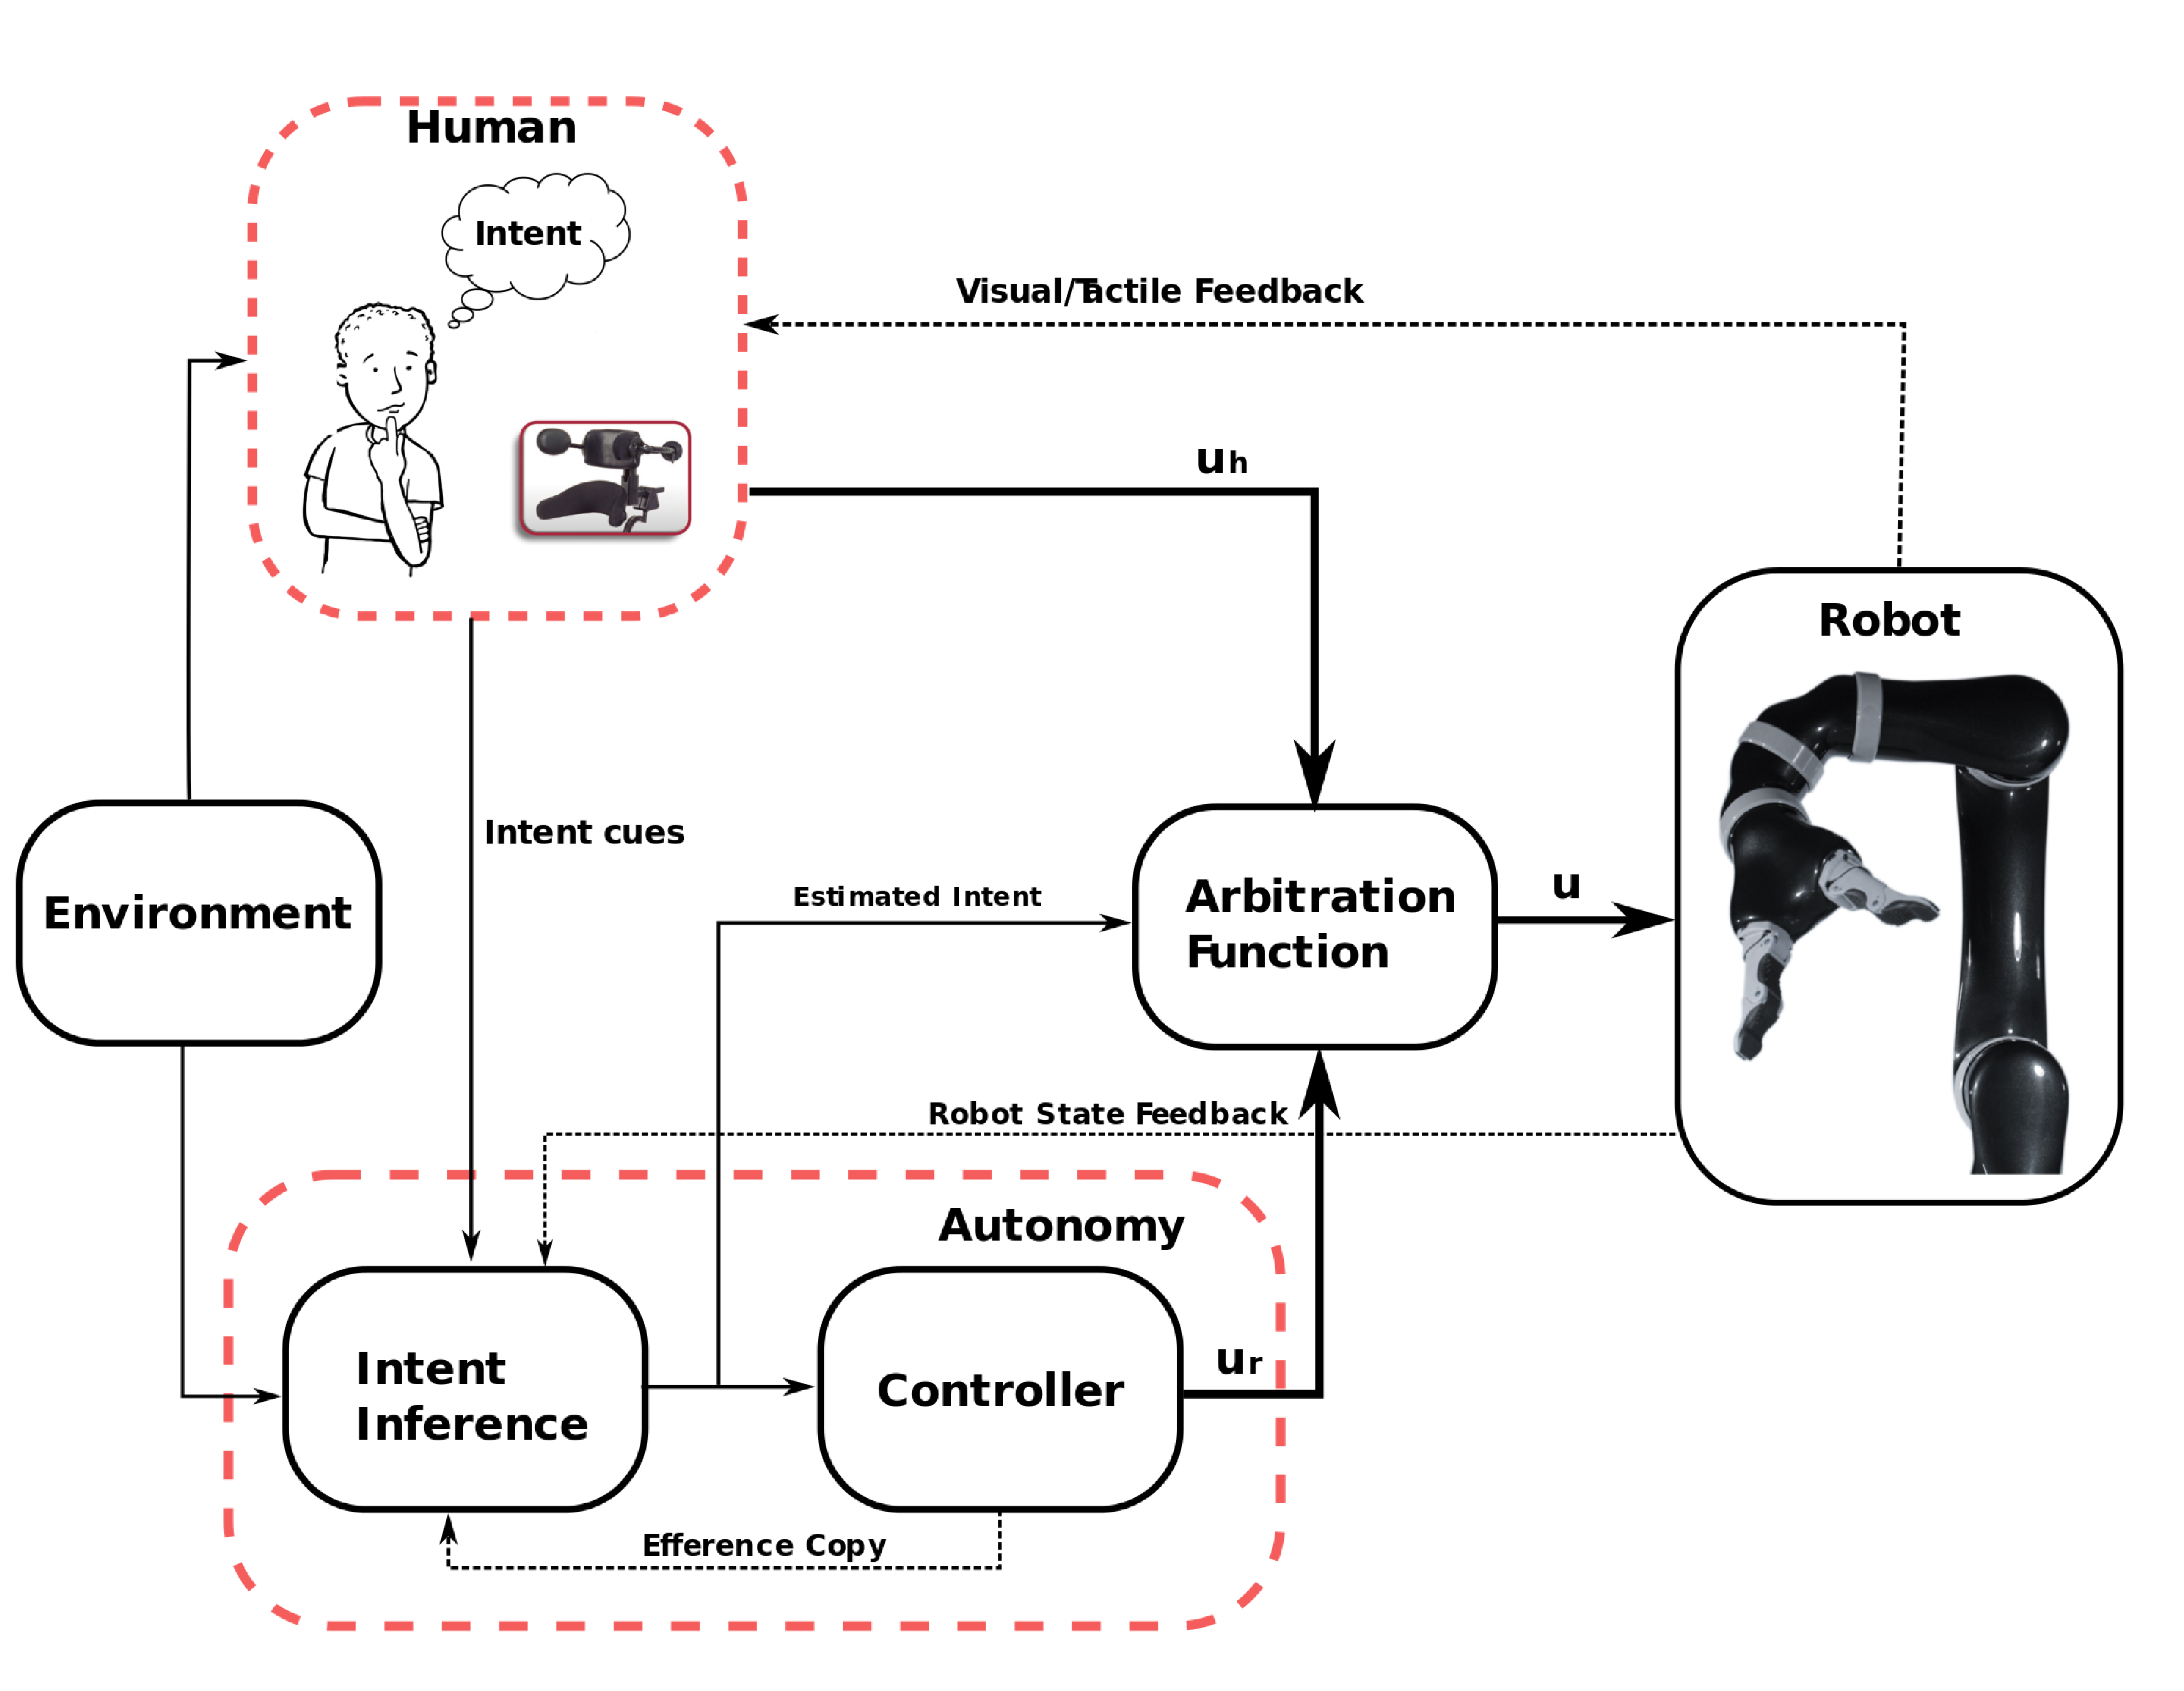
\includegraphics[keepaspectratio, width = 0.5\textwidth, center]{./figures/Fig1.eps}
	\caption{Illustration of the core components of a shared control architecture. $\boldsymbol{u}_h$ denotes the human control command, $\boldsymbol{u}_r$ denotes the autonomy control command and $\boldsymbol{u}$ is the final control command issued to the robot. Note the presence of different feedback channels between the components that can lead to highly coupled and nonlinear human-robot interactions. }
	\label{fig:shared_control}
\end{figure}
\subsection{Components of Shared-Control System}
A shared-control human-robot system consists of several different components that constantly interact with each in highly coupled and nonlinear fashion. Some of the salient components are 
\begin{enumerate}
	\item \textbf{Human}: Although task accomplishment is a joint responsibility  in a shared-control system, the robot is used \textit{by} a human to realize his/her own intent. For example, a motor-impaired person might use a shared-control wheelchair for navigation purposes or a robotic arm for performing activities of daily living. The human typically teleoperates a robot via a control interface according to their underlying intent. The human also receives input from the environment and sensory feedback from the physical robot as well which will further inform the actions that they perform.
	\item \textbf{Autonomy}: In Figure~\ref{fig:shared_control} autonomy consists of two sub-components:
		\begin{enumerate}
			\item Intent Inference: In order for the autonomy to decide when and how to intervene in task execution, it needs to have a good idea of what the user's intentions are. Therefore, intent inference mechanism play a crucial role in the success of shared-autonomy. In many cases, intent inference is a mechanism by which the system is trying to infer the human's hidden internal state. For example, in the context of shared-control assistive manipulation, intent inference may be cast as a problem of inferring the human's intended goal. The intent inference engine may rely on intent cues provided by the human, environmental cues,feedback from the robot and efference copy of the autonomy command from the robot controller to estimate the user's intent. 
			\item Robot Controller: The robot controller generates the autonomy command according to some policy which may be hand engineered or learned from data. The intent estimate provided by the intent inference module will further inform the synthesis of appropriate control commands by the controller. 
		\end{enumerate}
	\item \textbf{Arbitration Function}: The arbitration function is a critical component which decides how the control is shared between the human and the robot. It takes the human control command and the autonomy control command as inputs and arbitrates between them using a predefined or an adaptive criteria. The arbitration criteria may depend on the intent estimate from the intent inference engine and other factors such as environmental cues to produce a final control command that is issued to the physical robot. 
	\item \textbf{Robot}: The physical robot receives the final control command from the arbitration module and affects change in the environment and provides feedback to the human and the autonomy. 
\end{enumerate}
\subsection{Argument for Information Theoretic Approaches}
It is obvious from Figure~\ref{fig:shared_control} that the different components within a shared-control system interact with each other in a highly coupled and nonlinear fashion giving rise to intricate human robot interactions\footnote{Appendix~\ref{sec:appendix} contains the mathematical details of how the different components interact.}. Analysis of the dynamics of each of the components in isolation might ignore the subtle and complex nature of the interactions and other important global properties of these systems. analysis of information transfer between the various components can shed light on the how humans and robots cooperate and coordinate during task execution, the need for training and the existence of bottlenecks that can have a detrimental effect on seamless human-robot interaction. It is also obvious that if any of the connections between the different components are broken they can result in suboptimal performance or in some cases even failure of the shared-control system. 

Researchers have already identified how human robot interactions are facilitated via transfer for information via various channels that exist in these systems\footnote{For example, some of the information transfer channels in Figure~\ref{fig:shared_control} are \textit{a)} Human to Autonomy \textit{b)} Robot to Human.}. In \cite{gold2009information}, Gold proposes an information theoretic pipeline model for HRI  identifies various information channels that exist in the context of a human-robot system. Gold explicitly states that `\textit{the analysis in this paper only consider which information channel tends to be larger than others}' and that his `\textit{hope is that other researchers might be interested in considering HRI from an information theoretic perspective}'. In the spirit of Gold's work, in our paper we present a thorough investigation of information transfer between different components in a shared-control system. 

%Appendix can have generic equations showing the interdependence of human and robot dynamics are. 
%Analysing each component separately might be shortsighted approac and can miss out on the deeper interactions between the various subsystems. 
%
%human, intent inference, autonomy, arbitration, final control command and forward propgation of dynamics. 

\section{EXPERIMENTAL EVALUATION}\label{sec:exp_setup}
The information theoretic analysis of human-robot interaction was performed on data collected on two different shared-control assistive robotic manipulation tasks. For this study eight subjects were recruited. All participants gave their informed, signed consent to participate in the experiment, which was approved by Northwestern University's Institutional Review Board. 
\subsection{Hardware, Tasks and Protocol}
The experiments were performed using a MICO 6-DoF robotic arm (Kinova Robotics, Canada). The subjects operated the robot using two different control interfaces: a 2-axis joystick and a switch-based headarray. Two different reaching tasks were performed. The intent inference mechanism was based on a dynamic neural field approach~\cite{gopinath2018dynamic} to maintain and update the probability distribution over the discrete goals in the environment. The autonomy command was generated using a potential field based approach~\cite{khatib1986real}. The shared-control paradigm relied on a blending-based system in which the final control command issued to the robot was a linear combination of the human control command and the autonomy control command~\cite{dragan2013policy}. The blending factor was a linear piecewise function of the robot's confidence in its estimation of human intent (mode of the probability distribution over goals). 

\subsection{Data Analysis}

In this paper, we considered the information transfer in two specific information channels namely, a) Human to Intent inference, which would shed light on whether the human was able to coordinate and provide intent-expressive control commands and b) Robot to Human, which would reveal how the robot was able to convey its intent and how aware the human was to such cues. For this purpose, during every trial we recorded time series data corresponding to the user control command, the autonomy control command, goal probabilities and the blending factor. 

All data analysis was performed using the JIDT MATLAB toolbox~\cite{lizier2014jidt}. Since all the signals of interest in our work were continuous, we relied on the KSG estimators for transfer entropy computations. The embedding dimensions for both source and destination were determined by considering the active information storage in the both signals. Significance testing was performed via surrogate analysis in which one of the signals was scrambled in time to destroy any potential temporal correlation and structure. (more to be added as I generate results). 
%
%Talk about assistive robot manipulation. Tasks. Data recorded. What are we analysing for (what type of interactions). Anchor the symbols used in the previous section to concrete quantities specific to this setup. list all parameters and quantities in a table. 
%Qualititatively we observed intersubject variability. Some were timid/cautious, aothers were aggressiuve, Some paid attention to what the robot was dong and others were confident in their own abilities. 
%Add picture from Auro2017 paper. Shared control robot paradigm. We record time series of human control commands, autonomy control commands, goal probabilities. As a measure of robot to user we look at TE from autonomy command seen by the human to human control command. In opposite direction, we are interested in how the user was able to transfer intent information via the human control command. Human control command to goal probability associated with intended goal. Used JIdt. Multivaraite Kraskov was chosen, Embedding dimension was chosen by check for a range of embedding values and looking at the peak of active informtaion storage. Surrograt analysis was performed with 1000 iterations for each time series. Correlation analysis between TE and performance metric was also performed. To see that when there is high TE, performance is better due to better mutual understanding 
\section{RESULTS}\label{sec:results}
\section{DISCUSSION}\label{sec:discussion}
\section{CONCLUSION}\label{sec:conclusion}
\section*{Appendix}\label{sec:appendix}
Here we describe the coupled nonlinear interactions between the different components of a shared-control system in mathematical terms. Table~\ref{tbl:vars} lists all the relevant variables and parameters that correspond to the components depicted in Figure~\ref{fig:shared_control}.
\begin{table}[t]
	\centering
	\caption{Relevant variables and parameters corresponding to the different components of a shared-control system. The time dependence of each variable is omitted for the sake of brevity.} 
	\begin{tabular}{|p{3cm}|p{3cm}|}
		\hline
		\textbf{Variable/Parameter} & \textbf{Description}  \\ \hline
		$\boldsymbol{u}_h$ & Human Control Command \\ \hline
		$\boldsymbol{u}_r$ & Autonomy Control Command \\ \hline
		$\boldsymbol{u}_f$ & Final Control Command \\ \hline
		$\theta_h$ & Human Internal State (Intent) \\ \hline
		$\theta_r$ & Robot state \\ \hline
		$\theta_e$ & Environment State \\ \hline
		$\boldsymbol{p}(\theta_h)$ & Belief over Human Intent for Intent Inference \\ \hline
		
	\end{tabular}
	\vspace{.2cm}
	
	\label{tbl:vars}
	\vspace{-.5cm}
\end{table} 

The functional relationships between the components can be expressed in mathematical terms as follows.
\begin{align*}
	\boldsymbol{u}_h^t &= f_h(\boldsymbol{u}_r^t;\theta_h^t,\theta_r^t,\theta_e^t ) \\
	\boldsymbol{p}^t(\theta_h) &= F(\boldsymbol{p}^{t-1}(\theta_h); \theta_h^t,\theta_r^t,\theta_e^t) \\ 
	\boldsymbol{u}_r^t &= f_r(p^t(\theta_h);\theta_r^t,\theta_e^t) \\
	\boldsymbol{u}_f^t &= \beta(\boldsymbol{u}_h^t,\boldsymbol{u}_r^t; \boldsymbol{p}^t(\theta_h))\\
	\theta_r^t &= H(\theta_r^{t-1}, \boldsymbol{u}_f^t)	
\end{align*}
in which $f_h$ corresponds to the human policy or plan that the user follows to execute the control commands. $f_h$ may be deterministic or stochastic and can be approximated using domain knowledge or learned from data. $f_r$ corresponds to the robot policy. In this paper, we rely use a potential field-based approach to generate $f_r$. $F$ specifies the update rule for the time-evolution of the belief over the hidden human internal state (underlying intent) denoted by $\boldsymbol{p}(\theta_h)$. $\beta$ is the arbitration function that fuses the human control command and the autonomy control command to produce a final control command $\boldsymbol{u}_f$ as informed by the intent estimate. The robot state $\theta_r$ is updated via $H$, which may be interpreted as the kinematic or dynamical equations of motion for the robot. Without loss of generality each of these functions maybe nonlinear and may dependent on variable values from past time indices as well. The highly coupled nature of interaction is obvious from the above equations. 

%\balance	
\bibliographystyle{IEEEtran}
\bibliography{references}





\end{document}
